\section{Abstract}\label{abstract}

The meaning we derive from our experiences is not a simple static
extraction of the elements but, rather, is largely based on the order in
which those elements occur. Influential theoretical models propose that
the encoding of sequences of elements (or items) may be supported by
interactions between high and low frequency brain rhythms, such that
items within an episode are represented by neural cell assemblies firing
at higher frequencies (i.e.~gamma) and their relative sequential order
is coded by the specific timing of firing with respect to a slower
frequency rhythm (i.e.~theta). Using magnetoencephalography (MEG) to
record neural oscillations during episodic sequence memory formation in
humans, we provide evidence that items in different ordinal positions
within a sequence exhibit relatively greater gamma power along distinct
phases of an underlying theta oscillation. Furthermore, this segregation
is related to successful memory for the order of the items. These
results provide compelling evidence that memory for order, a core
component of an episodic memory trace, capitalizes on the seemingly
ubiquitous physiological mechanism of theta-gamma phase-amplitude
coupling.

\section{Introduction}\label{introduction}

While many aspects of our cognition and behavior, including language
processing, spatial navigation and episodic memory, share the
requirement to represent, encode and retrieve temporal sequences of
events, how the brain accomplishes this is still not well understood. It
is has been known for decades that two stimuli that activate
interconnected neurons can result in long-term potentiation (LTP) of the
bridging synapse \autocite{bliss_long-lasting_1973}, thus supporting an
association between the two, and compelling new research has provided
causal evidence for a link between LTP and associative memory formation
\autocite{nabavi_engineering_2014}. However, the model of long-term
potentiation in its current form is not viable for stimuli (or neurons)
whose activation is separated by more than \textasciitilde{}300 ms, and
unarguably, much of what we encode and remember is separated by temporal
gaps at least an order of magnitude large than this. Thus, a central
issue in understanding temporal sequence learning is how the brain can
bridge and relate stimuli that are encountered across seconds or
minutes.

To deal with this conundrum, mechanistic models of sequence encoding
posit that the temporal coding of sequences can be supported by neural
oscillations
\autocites{lisman_storage_1995}{jensen_hippocampal_1996}{lisman_-_2013}{jensen_physiologically_1996}{koene_first-first-out_2007},
or rhythmic fluctuations in neuronal excitability (see
\textcite{buzsaki_neuronal_2004} for review). One influential model of
sequence encoding \autocites{lisman_storage_1995}{lisman_-_2013}
hypothesizes that individual items are represented by largely
non-overlapping neural cell assemblies that, when activated, fire in
high frequency bands (i.e.~gamma: \textgreater{}30 Hz), while the
relative sequential order of those items is coded in a temporally
segregated manner along the phase of an underlying slower rhythm
(i.e.~theta: \textasciitilde{}3-8 Hz). It follows then that during the
encoding of a sequence, the current item is represented and encoded by
transient higher frequency activity, while the relative position of each
item in a sequence may be coded by the relative phase of a lower
frequency oscillation (referred to as `phase coding'). Theoretically,
phase coding allows the temporal segregation of activity supporting
individual items that are encountered at different times across an
experience, and critically may also permit temporally extended
experiences to be represented in a time-compressed manner
\autocite{jensen_physiologically_1996} (\textasciitilde{}100-300 ms
cycles of neuronal activity).

There is ample evidence that modulation of gamma power by theta phase
(i.e.~phase-amplitude coupling or `PAC') is important for learning and
memory formation
\autocites{axmacher_cross-frequency_2010}{tort_thetagamma_2009}{friese_successful_2013}{fuentemilla_theta-coupled_2010}[gamma\_2014]{lega_slow-theta}
as well as other cognitive processes
\autocites{canolty_high_2006}{giraud_cortical_2012}{szczepanski_dynamic_2014}.
However, to date, there is little evidence that theta phase coding, or
the segregation of item-specific neural assemblies on distinct phases of
an underlying theta oscillation, serves as a mechanism for human
sequence memory encoding. We set out to test this fundamental question
by presenting participants with six-item sequences each consisting of
pictures of trial-unique objects that were embedded on a repeating
background colored frame (Figure 1a) while recording brain activity
using magnetoencephalography (MEG). The colored frame defined each
six-item sequence as the color switched every six trials. We later
tested participants sequence memory by asking them to recognize the
correct order of two previously presented objects during retrieval.
Thus, we could ask whether gamma power associated with each item in a
sequence (positions 1-6) is relatively biased towards distinct phases of
theta (i.e.~phase coding). Importantly, we also assessed whether theta
phase coding was behaviorally relevant by examining phase coding effects
during both successful and unsuccessful temporal order encoding.

\section{Methods}\label{methods}

\subsubsection{Participants}\label{participants}

Twenty healthy right-handed native English speakers (4 males, age range:
21-35, mean age: 28) recruited from New York University and the greater
New York metropolitan area participated in the MEG experiment. The study
was approved by the University Committee on Activities Involving Human
Subjects and all participants gave informed written consent. We excluded
two subjects whose performance on the order memory test was not
significantly different from chance (50\%, using binomial test) and one
subject who did not complete the study due to drowsiness. We excluded
these participants, leaving 17 subjects for the MEG analyses.

\subsubsection{Materials}\label{materials}

Stimuli consisted of 576 gray-scale pictures of objects collected from
various online sources. Some examples of stimuli can be seen in the main
text (Figure 1). Colored borders for the objects were generated by
selecting 24 unique colors from a color continuum ranging from
{[}0,0,0{]} to {[}255,255,255{]} RGB values. Colors were manually chosen
to be maximally distinct from each other.

\subsubsection{Design and Procedure}\label{design-and-procedure}

\emph{Encoding}. During encoding, participants made pleasant/unpleasant
decisions on trial-unique objects that were paired with a colored
background frame. Specifically, participants were instructed to imagine
each object in the color of the background frame and press a button to
indicate whether or not the combination was pleasant. We chose to use
this encoding task to encourage participants to associate the color and
object, since attention to the context (i.e.~color) was critical to our
hypothesis. To promote successful temporal order memory, we additionally
instructed participants to associate neighboring objects together by
imagining them interacting with each other. Subjects were instructed to
perform this task irrespective of the color changes between some of the
items. Pilot data indicated that this instructional manipulation was
critical to achieving above chance temporal order memory performance in
a majority of our participants.

During the encoding task, the background color frame remained the same
for 6 consecutive trials (i.e.~a `sequence') and then switched to a new
color. There were 6 sequences (totaling 36 objects) in each encoding
block and 16 encoding/test blocks across the experiment. Each object was
on the screen for 2.5 seconds, followed by a 2 second inter-trial
interval (ITI) and a .5 second fixation period. The timing of the task
was fixed (i.e.~not jittered). During the ITI and fixation period, the
color frame remained on the screen.

\emph{Temporal order memory test.} After each study block, we tested
temporal order memory. We used this temporal order test as a proxy for
probing intact sequence memory. In this test, two previously studied
objects were presented side by side (with the previously colored
background frame now gray). Participants were asked to indicate which of
the two objects appeared first (earlier) in the sequence and rate their
confidence using a 4 alternative forced choice design. Thus, there were
four possible responses during the test: high confidence correct order,
low confidence correct order, high confidence incorrect order and low
confidence incorrect order. The tested objects always occurred in the
2nd and 6th position within a sequence and all tested object pairs were
separated by 3 intervening trials during encoding. The test was
self-paced with a mandatory .5 second fixation period between each test
trial.

\subsubsection{MEG recordings and data
processing}\label{meg-recordings-and-data-processing}

MEG data were recorded using a 157-channel whole-head axial gradiometer
system (KIT, Kanazawa, Japan). Three reference channels seated above the
MEG system were also recorded and used to remove ambient electromagnetic
environmental noise from the data. MEG data were acquired in DC with a
sampling rate of 1000 Hz, a low pass filter at 200 Hz and a notch filter
at 60 Hz to remove line noise. To measure head position, 5
electromagnetic coils were attached to a participant's head during
recording. Coil locations were determined by registering scalp coil
positions with 3D digitized head shape data (software: Source Signal
Imaging, Inc.; hardware: Polhemus, Inc.), which was collected before MEG
recording. The anatomical locations used to register the coils with the
head shape data were the nasion and the left and right periauricular
points. The coils were localized to the MEG sensors at the beginning and
end of the experiment.

MEG data were preprocessed as follows: raw MEG data were loaded into
MATLAB (version 7.10, Mathworks) and malfunctioning channels (average
per subject: \textasciitilde{}2) were immediately removed and
interpolated with the average of its nearest neighbors. Then, data were
denoised using a time-shifted principal components analysis approach
(temporal shift parameter = 100ms), which removed ambient environmental
noise using 3 reference channels \autocite{de_cheveigne_denoising_2007}.
The remaining preprocessing steps utilized the Fieldtrip M/EEG software
package \autocite{oostenveld_fieldtrip:_2010} and custom MATLAB scripts.
The data were band-pass filtered (default settings in eegfilt.m) from
1-100 Hz. Then, the data were epoched from -4 to 4 seconds surrounding
trial onset to assure adequate time for spectral estimation of both pre-
and post-stimulus activity. The epochs were downsampled to 500 Hz to
speed processing time in later steps. Finally, to facilitate
interpretation of topographic plots, we transformed the MEG data from
axial to planar gradient. One advantage of this linear transformation is
that planar signal amplitude is typically largest directly above the
source, whereas axial signal amplitudes are typically maximal on either
side of the neural source of the signal. This transformation was
performed for all topographic analyses, but not the source-space
analyses.

After preprocessing, the MEG data were examined for artifacts. The
artifact rejection approach we took was three-fold: First, excessively
noisy trials and channels were removed using Fieldtrip's visual artifact
rejection `trial summary' feature. Specifically, channels and trials for
which the across-trial variance exceeded 3 standard deviations from the
mean were identified and removed from the analysis. Then, independent
component analysis was implemented to remove components related to eye
blinks, eye movements, and heartbeat-related artifacts. Finally,
remaining trials were visually inspected and epochs containing any
remaining artifacts were removed from the dataset. The group average
proportion of trials removed due to artifacts was
\textasciitilde{}8.6\%.

\subsubsection{Time-Frequency Power
Analyses}\label{time-frequency-power-analyses}

A time-frequency analysis was performed for each epoch (-4 to 4 seconds,
50 ms sliding window, zero-padded) using a morlet wavelet approach
(number of cycles=6), estimating spectral power from 1 to 100 Hz in
steps of 1 Hz. This analysis resulted in time-frequency spectrograms
representing oscillatory power for each time-frequency-sensor point for
each trial and each subject. This relatively long epoch window allowed
us to analyze data during the `stimulus on' period (0 to 2.5 seconds) as
well as the inter-trial periods (-2.5 to 0 seconds) while avoiding edge
artifacts particularly in the low frequencies.

\subsubsection{Cross-Frequency Coupling
Analyses}\label{cross-frequency-coupling-analyses}

Phase-amplitude cross-frequency coupling (PAC) was estimated as follows
for each trial for each sensor and subject. The algorithm to compute the
PAC `modulation index' (referred to as MI or coupling values/estimates)
was taken from \textcite{tort_measuring_2010}. First, to compute gamma
amplitude, raw MEG time-series (for each trial/sensor) was filtered from
70-100 Hz, which was determined by frequencies that showed a peak in the
spectral power distribution (Supplemental Figure 1). The envelope was
then computed by taking the absolute value of the Hilbert Transform of
the filtered time-series. To compute theta phase, the raw data was
filtered from 3 to 8 Hz in steps of 1 Hz resulting in 5 filtered
time-series (i.e.~3-4, 4-5, etc.). We filtered in steps of 1 Hz instead
of the range of the band (3-8 Hz) because we wanted to minimize the
possibility that changes in the peak frequency of the theta band could
explain our findings. Phase was computed for each of the 5 filtered time
series by taking the angle of the Hilbert transform of the filtered
signal. Then we binned gamma power by theta phase (18 bins) during
stimulus presentation (0-2.5 seconds), now averaging across the 5 theta
sub bins, resulting in a single theta-binned gamma histogram for each
trial. We then normalized the distributions, such that the power of each
histogram summed to one. Finally, we computed Kullback-Leibler
divergence for each theta-binned gamma distribution and divided by the
log(18) i.e.~the number of phase bins.

In order to determine statistical significance of the coupling values,
we employed a permutation procedure \autocite{canolty_high_2006}. For
each trial, we recomputed the coupling analysis described above, but
circularly shifted the time-series of phase values by a random interval
greater than 500 samples (i.e.~the sampling rate, 1 second). For each
trial (and theta phase sub-bin), we repeated this phase-shifting process
100 times to derive a null distribution of coupling values. We then
converted the coupling estimates to statistical values (z-statistics).
To calculate within-subject statistics, we computed a t-statistic across
trials (averaging across theta-sub bin, i.e.~one value per trial) for
each sensor and subject. Then, to calculate group-level statistics, we
computed a t-statistic across subjects for each sensor.

\subsubsection{Fitting Theta-Gamma Coupling Estimates to the
Model}\label{fitting-theta-gamma-coupling-estimates-to-the-model}

Our initial hypothesis was that as items are maintained in and
integrated into working memory, additional gamma cycles would be
concatenated along the phase of theta 19. To simulate this hypothesis
and test for this pattern in our data, we generated theta (4 Hz)
sinusoidal waves (10 cycles to mimic our 2.5 second stimulus
presentation), adding 1 to 6 cycles of a gamma rhythm (85 Hz) per theta
cycle. The 6 different simulations represented our hypotheses for the 6
positions within a sequence. We then computed the predicted coupling
score (i.e.~modulation index) for each of these simulations. Due to an
increase in the width of the distribution of gamma over theta as
function of sequence trial position, our simulation predicted linearly
decreasing coupling values across sequence positions (see Figure 1b and
c for visual depiction).

To test for this pattern of broadening gamma over theta in our data, we
performed a linear regression on the trial-wise estimates of theta-gamma
coupling. The predictor (independent) variable was our simulated
hypothesis (described above) and the dependent variable was a vector of
observed coupling estimates. To construct the vectors of coupling
values, for each trial/sensor/subject, we averaged together the coupling
estimates across theta sub-bins so that there was a single coupling
value per trial. We then performed a separate linear regression analysis
(independent: model-predicted coupling value, dependent: trial-wise
coupling estimate) for each sensor/subject, resulting in subject-level
topographic statistical maps (t-values) representing the fits of our
model to the empirically observed coupling estimates. Then to compute
group-level statistics, we computed a t-statistic across subjects for
each sensor (see Figure 1d). To correct for multiple comparisons, we
derived a statistical threshold based on the size of a cluster of
sensors compared to what one might expect by chance. For each
sensor/subject, we shuffled the trial labels (1000 times) and then refit
the model. Then, we recomputed cluster sizes on each iteration to build
a null distribution of maximum cluster sizes expected by chance and only
retained clusters exceeding p\textless{}.05 of the null distribution of
cluster sizes. Only clusters of sensors that exceeded this threshold
were further analyzed.

To control for power differences across a sequence as a potential
confounding factor for the analyses described above, we performed a
second regression analysis where first, a general linear model with
theta and gamma power (as separate predictor variables) was constructed
and regressed against the coupling estimates. We then refit our model
(i.e.~decreasing coupling by sequence position) to the residuals of this
model. Thus, any explanatory power that theta or gamma power had on
theta-gamma coupling was removed. The result of this analysis is plotted
in Supplemental Figure 4.

\subsubsection{Theta-Gamma Model Source Localization
Analysis}\label{theta-gamma-model-source-localization-analysis}

A linearly-constrained minimum-variance beamformer analysis
\autocite{van_veen_localization_1997} was performed to estimate neural
sources of the decreasing theta-gamma coupling by sequence position.
Briefly, this technique utilizes an adaptive spatial filtering algorithm
designed to estimate sources of neural activity originating from a
spatial location in the brain given a particular topographic
distribution of MEG activity by applying a unit gain constraint to the
spatial location of interest and minimizing the contribution of all
other sources. First, each subject's data was registered to a canonical
structural MPRAGE brain from the FSL software package
\autocite{jenkinson_fsl_2012}. This was achieved by aligning anatomical
landmarks (nasion, left/right periauricular points) from digitized head
shape data to the structural brain image for each subject. To estimate
source-space time-series data, we used a combination of source analysis
script from the Fieldtrip software package as well as custom MATLAB
scripts. A semi-realistic head model was constructed following methods
described by \emph{ADD THIS REFERENCE} Nolte et al (2003). Then, using
the MEG data from all trials (irrespective of sequence position), a
common spatial filter was estimated for each point in a three
dimensional grid representing potential neural source locations with 1
centimeter spacing between points. The result of this analysis was a
vector of spatial weights (1 x 157, i.e.~the total number of MEG
sensors) mapping the contribution of each sensor's activity to a
particular grid (i.e.~brain) location. Then, to derive source-space time
series for each trial (-1 to 3.5 seconds), the matrix of sensor-level
time series (157 sensors x 2251 time points for each trial) was
multiplied by the spatial weight matrix, resulting in a single time
course for each source location for each trial.

Once the all the sensor-level data was projected into source space, we
performed an analysis very similar to the sensor-level theta-gamma model
fit analyses described above. For each trial (during stimulus
presentation, 0 to 2.5 seconds) and source-space location, we bandpass
filtered the data in the high gamma band (70-100 Hz; using default
filter settings of eegfilt.m) and computed gamma amplitude by taking the
absolute value of the Hilbert transform of the filtered signal. Then, we
derived the theta phase time course by bandpass filtering the data in
the theta frequency range (3-8 Hz; using default filter settings of
eegfilt.m) and then computed the angle of the Hilbert transform of the
filtered signal. The remainder of the analysis was identical to the
sensor-level theta-gamma model fitting analyses described above.
Briefly, for every subject, we computed theta-gamma coupling for each
trial/source-space point and fit the theta-gamma coupling source-space
point to our model of decreasing theta-gamma coupling as a function of
sequence position. Then, to compute group-level statistics, we computed
t-statistics across subjects for every source-space point. The final
product was a 3D source-space statistical map of t-values representing
the group reliability of the fit of theta-gamma coupling to our model of
decreasing coupling across sequence positions. Note that there is
typically a center bias for beamformer source localization when a source
is localized without respect to a baseline (i.e.~pre-stimulus period or
another condition). Given that the regression analysis we ran is a
linear contrast across sequence positions, this potential confound is
likely not a contributing factor.

\subsubsection{Phase Analyses}\label{phase-analyses}

We hypothesized that for items in different sequence positions, gamma
power would be biased to different phases of theta, particularly when
temporal order was successfully encoded. To test this, for each trial,
we computed histograms of gamma power binned by theta phase (18 bins;
power and phase computations are described above in Cross-frequency
Coupling Analyses section) for each sensor. We then averaged across
clusters of sensors that displayed a significant fit to our model
(i.e.~decreasing coupling by sequence position), which resulted in two
clusters (a left lateral cluster and a left posterior cluster), and then
sorted sequences by subsequent temporal order memory. To test whether
the theta-binned gamma distributions differed by sequence position, we
used a Watson-Williams multi-sample test for equal means implemented
from the Circular Statistics Toolbox for MATLAB
\autocite{berens_circstat:_2009}. This test is effectively a one-way
ANOVA for circular-linear data. To compute significance of the
interaction between position and sequence memory, we used a
Harrison-Kanji Test, a circular implementation of a two-way ANOVA. It
should be noted that all phase analyses described in this section were
statistically tested using circular-linear tests unless otherwise
specified.

In a follow up analysis, we then averaged the trials into 3 bins by
sequence position: 1\&2 (early), 3\&4 (middle) and 5\&6 (late). Finally,
we averaged the data across subjects. The result of this analysis was 6
histograms (for each cluster of interest) of gamma power binned by theta
phase for early, middle and late sequence trials and for sequences where
later temporal order was correct and incorrect (plotted in Figure 3).

To compute theta phase locking (also known as `inter-trial' phase
coherence), we followed methods outlined in 64 (see Figure 3c in the
referenced paper). Briefly, for each trial, we filtered the data at the
theta frequency. Then, we computed the Hilbert transform and normalized
the resulting complex vectors to remove the amplitude component.
Finally, for each time point, we computed the phase locking value by
averaging the normalized vectors across trials for a given condition for
each subject.

\section{Results}\label{results}

\begin{figure}
  \centering
  \includegraphics[width=\textwidth]{figures/chapter3_figure1.eps}
  \caption[Theta-gamma coupling analysis and model fits.]{A. Schematic of the sequence encoding paradigm.  Participants viewed a series of trial-unique objects (36 per block) embedded on a colored frame which periodically switched every 6 trials.  After each block, temporal order memory was probed by presenting two items studied within the same color and asking which of the two occurred earlier in the sequence. B. Model of theta-gamma phase coding hypothesis. In this model, items (represented in gamma) encountered in the same color are concatenated along the theta phase.  At switches in color, item representations are hypothesized to be removed.  C. Expected pattern of theta-gamma coupling measure (MI: modulation index) across sequence positions derived from simulated hypothesis.  D. Group-level topographic statistical map (t-values, threshold t(16)>2.1, p<.05, cluster corrected using bootstrapping procedure) representing fit of model to across-trial theta-gamma coupling estimates. Two significant clusters of sensors emerged: 1) a left lateralized cluster and 2) a left posterior cluster. E. Group-level source space statistical map (t-values) representing fit of model to across-trial theta-gamma coupling estimates.  Coronal (left), axial (middle) and sagittal (right) views are shown.  Source space statistical map is thresholded at t(16)>3.22, p<.005, uncorrected. PHG = parahippocampal gyrus.  FG = fusiform gyrus.}
  \label{chapter3_figure1}
\end{figure}

\subsubsection{Sequence memory
performance}\label{sequence-memory-performance}

During each encoding-retrieval block, participants encoded six 6-item
sequences (for a total of 36 consecutive object stimuli) before being
tested for the temporal order of pairs of object stimuli from each
presented sequence. Behaviorally, temporal order memory for pairs of
object stimuli studied within a sequence (specifically positions 2 and 6
of a six-item train) was well above chance (\(\mu\) = .74, \(\sigma\) =
.12, chance was .5), confirming that temporal order encoding was
feasible (but not always attainable) in our task design which,
importantly, allowed us to compare successful to unsuccessful encoding
of sequences.

\subsubsection{Theta/gamma power and coupling during sequence
encoding}\label{thetagamma-power-and-coupling-during-sequence-encoding}

Before testing the critical hypotheses concerning whether theta-gamma
interactions are related to successful sequence memory formation, we
first characterized the distribution of spectral power in the MEG data
in a broad range of frequency bands (1-100 Hz) during stimulus encoding
(0 to 2.5 seconds), baseline corrected relative to a pre-stimulus time
period (-1 to 0 seconds), averaging power over time, trials, sensors,
and subjects. This quantitative analysis provides a global measure of
the frequency content of the signal and allows identification of
reliable peaks in the power spectra, since spectral peaks are necessary
for a meaningful estimate of phase - and ultimately a reliable estimate
of cross-frequency coupling \autocite{aru_untangling_2015}. We found
distinct peaks in the spectral power distributions in both the theta
(3-8 Hz) and high gamma (70-100 Hz) bands that were present during each
trial presentation as compared to a pre-stimulus baseline period (-1 to
0 seconds) (Supplemental Figure 1). Using these spectral power peaks to
constrain frequencies of interest, we next tested whether any reliable
relationship between theta and gamma oscillations were present in our
data using a well-characterized PAC measure that tests for the tendency
of power in a higher frequency to be biased towards any particular phase
of a lower frequency
\autocites{tort_measuring_2010}{tort_thetagamma_2009}. Using a
permutation-based bootstrapping technique (inspired by
\textcite{canolty_high_2006}; see Online Methods), we identified
significant theta-gamma PAC in a number of MEG sensors distributed
across the scalp (t\textgreater{}3.96, p\textless{}.001, Supplemental
Figure 2).

\subsubsection{Modulation of theta-gamma coupling by sequence
position}\label{modulation-of-theta-gamma-coupling-by-sequence-position}

Next, we asked whether theta-gamma PAC was modulated across items within
each event (6-item sequence). If items are temporally coded by gamma
power that is biased towards distinct phases of theta, then theta-gamma
coupling may be parametrically modulated as a function of an item's
position within a sequence. We hypothesized that the encoding of items
in the initial part of a sequence should be associated with a tight
theta phase - gamma amplitude relationship (and thus a high coupling
score) because a single item would be represented and maintained at a
particular phase on repeating cycles of theta
\autocites{jensen_hippocampal_1996}{jensen_hippocampal_1996}. However,
as subsequent items are encountered within a sequence, additional gamma
cycles (representing additional items) would become present and hence
result in the widening of the overall distribution of gamma power over
the phase of theta (see Figure 1b for schematic of the hypothesized
modulation by position). This would, somewhat counter-intuitively,
result in an overall reduction in our measure of theta-gamma coupling as
more items are added into the sequence. To, quantify this hypothesis, we
ran a simulation of theta-gamma coupling where, for each trial within a
sequence, additional gamma cycles (representing additional items in the
sequence) were concatenated along the phase of a theta oscillation. PAC
was then estimated on the simulated data. This verified our intuition
that if our hypothesis is correct, our PAC measure should linearly
decrease across trials when estimated separately for each trial within a
sequence (Figure 1c).

Based on the results of the simulation, we then examined the MEG data
for this pattern of decreasing theta-gamma PAC across each 6-item
sequence. For each position in the 6-item sequence, we estimated average
theta-gamma PAC during each stimulus presentation (0-2.5 seconds). Then,
using the pattern estimated by our simulated hypothesis as a predictor
variable (i.e.~a linear decrease in PAC across positions within a
sequence; Figure 1c), we performed a linear regression on the PAC
estimates to identify sensors that displayed the predicted pattern of
results. We found two clusters of sensors (left lateral and left
posterior) that reliably fit our model at the group-level (Figure 1d;
thresholded at \emph{t}(16) \textgreater{} 2.1, \emph{p} \textless{}
.05; cluster-corrected using permutation test procedure, see Methods).
To verify that this result was driven by our expected pattern, we then
extracted theta-gamma PAC estimates (as well as power estimates) from
sensors that showed a significant fit to our model and plotted the group
average theta-gamma PAC estimate for each sequence position. Visual
inspection confirms a linearly decreasing pattern across the sequence,
consistent with the PAC simulation (Supplemental Figure 3). While there
was a linear increase in theta power over sequence positions, regressing
out the power values (both theta and gamma) had virtually no effect on
the PAC model fits (See Supplemental Figure 4; \emph{F}(1,5332) = .002,
\emph{p} = .96) and thus do not appear to interact with the PAC effects.
In summary, we found that theta-gamma PAC decreased across items in a
sequence, consistent with the idea that sequence encoding may be
supported by the concatenation of gamma cycles at distinct, consecutive
phases of theta for each additional item in the sequence.

\subsubsection{Source localization of theta-gamma coupling decreases
over sequence
position}\label{source-localization-of-theta-gamma-coupling-decreases-over-sequence-position}

So far, we have provided evidence that theta-gamma PAC during object
sequence encoding decreases across sequential positions, consistent with
the notion that items in a sequence may be coded by gamma cycles aligned
sequentially along distinct yet consecutive phases of an underlying
theta cycle. Theoretical models
\autocites{jensen_hippocampal_1996}{jensen_hippocampal_2005} and
empirical research in humans
\autocites{dubrow_temporal_2014}{hsieh_hippocampal_2014}{jenkins_prefrontal_2010}{tubridy_medial_2011}{davachi_how_2015}{ezzyat_similarity_2014}
and rodents \autocites{fortin_critical_2002}{kesner_role_2002} all point
towards the hippocampus as being a structure that is critical for the
formation of temporal associations among items. In humans, fMRI and
intracranial EEG recordings have allowed for the precise
characterization of hippocampal signals in spatial resolution on the
order of millimeters. While MEG is well suited for fine temporal
analysis of brain activity, recent advances in source localization
methods have made it possible to localize sources of MEG activity to a
spatial resolution on the order of single centimeters, or even
millimeters \autocite{dalal_spatial_2007}. Additionally, a growing
number of papers
\autocites{attal_assessment_2013}{dalal_simultaneous_2013}{staudigl_theta_2013}
and simulations \autocites{mills_techniques_2012}{quraan_detection_2011}
argue that source localization of MEG signals is possible to subcortical
structures such as the hippocampus, however the parameters required to
accurately source localize deep structures is still controversial and
actively debated in the literature. Nonetheless, we applied best
practice and performed a source localization analysis on our MEG data.
To that end, we first estimated trial-level time series in source space
using a linearly constrained minimum variance beamformer approach (see
Methods). Then, using the same PAC method as used on the sensor-level
analyses described above
\autocites{tort_measuring_2010}{tort_thetagamma_2009}, we computed PAC
estimates for each trial and each source-space point (whole brain) and
then fit the trial-wise PAC estimates to the model generated by our
simulation (i.e.~decreasing PAC estimates across a 6-item sequence).
Thus, this analysis was nearly identical to the sensor-level analysis,
but performed on source-space time-series estimates throughout the whole
brain. Remarkably, the only region to reliably emerge from this analysis
was a region of the medial temporal lobe centered in the left
hippocampus (Figure 1e, \emph{t} \textgreater{} 3.19, \emph{p}
\textless{} .005; see Supplemental Figure 5 for other thresholds),
extending posteriorly to a region of the parahippocampal gyrus bordering
on the fusiform gyrus. This result is consistent with the suspected role
of the hippocampus and surrounding medial temporal lobe cortical regions
in sequence encoding
\autocites{dubrow_temporal_2014}{hsieh_hippocampal_2014}{jenkins_prefrontal_2010}{tubridy_medial_2011}
and is consistent with the idea that sequence memory may be supported by
an interaction between theta and gamma band activity in the left
hippocampus.

\begin{figure}
  \centering
  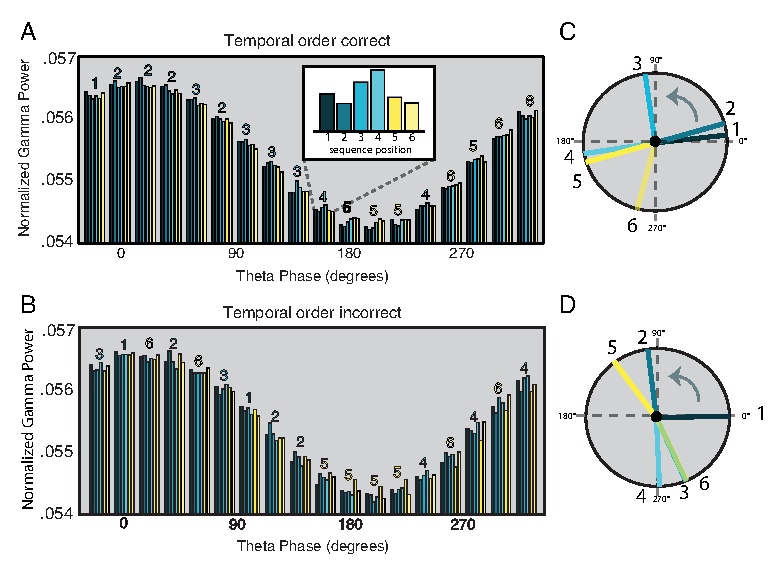
\includegraphics[width=\textwidth]{figures/chapter3_figure2.eps}
  \caption[Phase analysis of theta-gamma coupling by subsequent memory]{Phase analysis of theta-gamma coupling during sequence encoding plotted by position and subsequent temporal order memory for left posterior cluster of sensors.  A.  Theta-binned gamma distributions during successful sequence encoding.  Each color represents a distinct sequence position and the number above the bin represents the sequence position with the highest gamma power at that bin. The inset shows the relative pattern over sequence positions for a single phase bin.  B.  Theta-binned gamma distributions during unsuccessful sequence encoding.  C. Mean angle of theta-gamma coupling for each sequence position for successful sequence encoding.  The main effect (i.e. strong bias of gamma at all positions to the trough of theta) is removed to highlight the relative phase biases.  D. Mean angle of theta-gamma coupling for each sequence position for unsuccessful sequence encoding.}
  \label{chapter3_figure2}
\end{figure}

\subsubsection{Theta phase coding supports temporal sequence
encoding}\label{theta-phase-coding-supports-temporal-sequence-encoding}

While the sensor-level and source-space analyses described above
establish that theta-gamma PAC is modulated by position within a
sequence in a manner that is consistent with the idea that gamma-coded
objects are represented sequentially along the phase of theta, they do
not directly demonstrate that result. Indeed, one could imagine
alternative scenarios where the decreasing theta-gamma PAC pattern
across sequence positions could emerge - a simple example being that the
response pattern represents accumulating item representations without
the orderly representation of their temporal order.

Thus, we conducted additional analyses to directly test our central
hypothesis that objects encountered in different positions within a
sequence are coded at distinct and consecutive phases of theta. To that
end, we first extracted raw MEG data from the two clusters of sensors
that displayed a significant fit to the model derived from our simulated
data (Figure 1d). Separately for these two clusters of sensors, we
binned gamma power by the phase of theta (18 phase bins) to generate an
individual histogram for each trial (during stimulus presentation: 0-2.5
seconds; see Methods for details). We then averaged the theta-binned
gamma distributions for each cluster across all subjects, but separately
for trials in distinct sequence positions and also separately by
subsequent temporal order memory, as we reasoned that phase coding may
be present or robust only during successful sequence encoding.

Examining successfully encoded sequences first, in the left posterior
cluster of sensors we find a main effect of position on the distribution
of gamma power over theta phase (Watson-Williams Test: \emph{F}(5,96) =
16.04, \emph{p} \textless{} .0001) and, critically, the gamma power
distributions reflected the relative order in which the objects were
encoded (Figure 2a; Supplemental Figure 6). By contrast, for sequences
where order memory was later incorrect, we observed significant
differences in mean phase angle by position (Watson-Williams Test:
\emph{F}(5,96) = 5.26, \emph{p} \textless{} .0001), but the order of the
phase angles was scrambled relative to the actual order that the items
were experienced (Figure 2b). Critically, the memory by position
interaction was also significant (Harrison-Kanji Test: \emph{F}(5,196) =
15.79, \emph{p} = .01). Together, these results suggest that objects in
distinct ordinal positions within a sequence may be coded in gamma band
activity biased towards distinct, and ordered, phases of a theta
oscillation.

Another way to visualize this effect is to plot the relative phase
biases in polar coordinates. Thus, we transformed the theta-binned gamma
distributions into polar coordinates, now plotting the mean phase angle
of theta-gamma coupling for each sequence position separately for
sequences where order was later remembered and when they were forgotten,
after removing the main effect of coupling, which was centered at the
trough of theta. We see that, for sequences whose temporal order was
later remembered, the order of the angles across sequence positions
reflected the order in which the objects were encoded (Figure 2c),
whereas for incorrect sequences, the order of the angles is scrambled
relative to the actual encoding order (Figure 2d).

In the next analysis, we averaged the theta-binned gamma distributions
for the 6-sequence positions into 3 bins (1\&2, 3\&4, 5\&6) after
subtracting out the main effect of coupling. A statistical contrast of
each position bin relative to the average of the other two bins shows
that gamma power was preferentially higher at distinct phase bins of
theta (Figure 2c; \emph{t}'s \textgreater{} 2.1, \emph{p}'s \textless{}
.05). However, for sequences where the temporal order was later
incorrectly remembered, the relative distributions for each position bin
were comparatively flat, and there were no single phase bins where the
position bins were significantly different from each other (\emph{t}'s
\textless{} 2.1, \emph{p}'s \textgreater{} .05). Together, these data
are consistent with the idea that successful sequence encoding is
accompanied by a theta-gamma phase coding mechanism, whereby gamma power
associated with each sequential item is biased toward a distinct,
consecutive phase of an underlying theta oscillation.

\begin{figure}
  \centering
  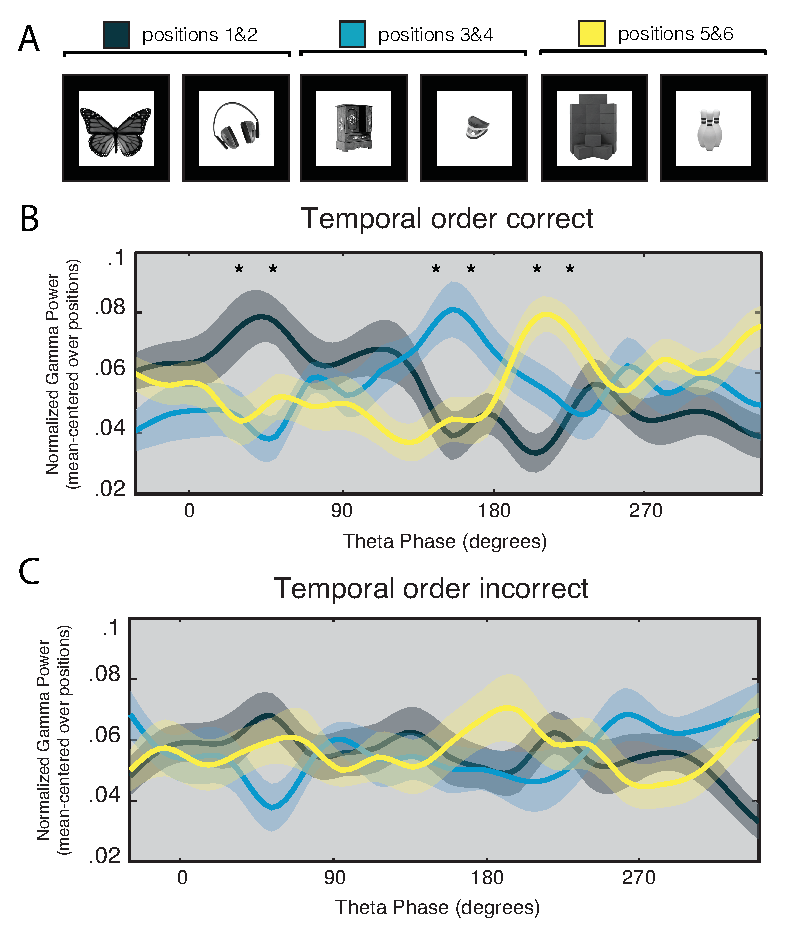
\includegraphics[width=\textwidth]{figures/chapter3_figure3.eps}
  \caption[Relative biases in gamma power over theta phase by sequence position and subsequent memory]{Relative biases in gamma power over theta phase by sequence position and subsequent memory.  A) Schematic representing our binning strategy.  We binned trials into early (1 and 2), middle (3 and 4), and late (5 and 6).  B) The distribution of gamma power over theta phase after removing the main effect of coupling for each sequence bin when temporal order was correct.  C) The same as B, but for sequences where order was incorrect. Stars represent phase bins where the statistical contrast (for example, early vs. the average of middle and late) was significant.  * p<.05}
  \label{chapter3_figure3}
\end{figure}

\subsubsection{Ruling out alternative
explanations}\label{ruling-out-alternative-explanations}

While the results reported here are consistent with a theta phase coding
account of sequence memory formation, it is important to rule out
alternative explanations for the data. Below, we outline a number of
control analyses aimed to test whether other features of the data could
explain the effects.

\emph{Temporal dynamics of gamma power and theta phase locking.} We
considered the possibility that variance in gamma power or theta phase
locking across sequence positions or memory conditions could explain the
phase coding effects. To test this, we analyzed the time course of gamma
power and theta phase locking separately by sequence position (binned
1\&2, 3\&4 and 5\&6) and by subsequent memory in the left posterior
cluster of interest that displayed phase coding. As can be seen in
Supplemental Figure 7 \& 8, transient stimulus-evoked gamma power and
theta phase locking stabilize by 500 ms post stimulus onset. There were
no differences in theta phase locking by position (0-500 ms:
\emph{F}(2,34) = .78, \emph{p} = .46, 500-2500 ms: \emph{F}(2,34) = .5,
\emph{p} = .61{]} and no differences by subsequent memory {[}0-500 ms:
\emph{F}(1,34) = 1.17, \emph{p} = .29; 500-2500 ms: \emph{F}(1,34) =
.04, \emph{p} = .96{]}. Gamma power also did not significantly vary by
sequence position (0-500 ms: \emph{F}(2,34) = .24, \emph{p} = .78;
500-2500ms: \emph{F}(2,34) = .13, \emph{p} = .87) and there was a trend
for greater gamma power in the forgotten sequences compared to the
remembered sequences early (0-500 ms) but not later (500-2500 ms) (0-500
ms: \emph{F}(1,34) = 3.12, \emph{p} = .09; 500-2500 ms: \emph{F}(1,34) =
.95, \emph{p} = .34). It's important to highlight that absolute gamma
power likely did not play a role in the phase coding effects we see
here, because for each trial, after computing the distribution of gamma
power over theta phase, the resulting distribution was normalized (to
sum to 1). This minimizes the likelihood that the phase coding effects
were somehow driven by gamma power differences across conditions.

\emph{Removing the stimulus evoked response.} One major concern when
performing cross-frequency coupling analyses is that the neural response
to the presentation of a stimulus could simultaneously result in a burst
of high-frequency activity and low frequency phase alignment over
trials. Thus, an effect that looks like a phase-amplitude interaction
may actually be driven by two independent processes with a common
driver. It is worth noting that a burst of high-frequency activity at
stimulus onset would need also be accompanied by (1) a predictable shift
in theta phase across each position in a sequence and (2) only do so on
successfully encoded sequences to fully account for our results.
Nonetheless, to rule out the possibility that our effects are in some
way driven by an evoked stimulus response, we reanalyzed the data
without the time window containing the evoked potential.

We then recomputed our phase coding analyses removing the first 500
milliseconds from each trial, which effectively removed the stimulus
onset response from the analysis. We found that both the decreasing PAC
over event positions (Supplemental Figure 9; including first 500ms:
\emph{t}(16) = 6.9868, \emph{p} = 3.0663e-06, excluding first 500ms:
\emph{t}(16) = 6.1015, \emph{p} = 1.5301e-05), as well as the phase
coding by subsequent order memory effects (Supplemental Figure 10;
excluding first 500ms - temporal order correct: Watson William's Test
\emph{F}(5,96) = 9.10, \emph{p} \textless{} .0001; temporal order
incorrect: Watson William's Test \emph{F}(5,96) = 6.42, \emph{p}
\textless{} .001; memory by sequence position interaction:
Harrison-Kanji Test: \emph{F}(5,196) = 11.03, \emph{p} = .025) were
still present and statistically robust.

\emph{Phase coding in the inter-trial interval.} As a further test to
rule out an evoked response confound, we ran these same analyses on the
time periods between each trial, the inter-trial intervals (ITI;
2500-5000 ms post stimulus onset), when participants were presumably
maintaining prior items and reinforcing associations between items.
Interestingly, we found that theta-gamma PAC was in fact stronger during
the ITI than the stimulus presentation interval (see Supplemental Figure
11a) and the phase coding by subsequent memory effects were still
present and robust (temporal order correct: Watson William's Test
\emph{F}(5,96) = 9.10, \emph{p} \textless{} .0001; temporal order
incorrect: Watson William's Test \emph{F}(5,96) = 9.09, \emph{p}
\textless{} .0001; position x memory interaction: Harrison-Kanji Test:
\emph{F}(5,196) = 8.02, \emph{p} = .07). However, the decreasing PAC by
sequence position effect was no longer present (Supplemental Figure
11b). This very intriguing result highlights that phase coding is
persistent even after the stimulus was removed from the screen, thus
ruling out the possibility that the evoked response is in someway
responsible for the phase coding pattern we observed.

\emph{Testing for systematic shifts in theta phase by sequence
position.} Another possible alternative explanation for our result is
that gamma power remains temporally fixed with respect to the onset of
the stimulus, but there is a systematic shift in theta phase as a
function of sequence positions, perhaps due to a reset in the phase of
theta caused by the stimulus presentation. To test for a mechanism of
this nature, we simulated sinusoidal time series at the theta frequency,
where the phase of theta systematically shifted over the sequence, and
then computed the cross-correlation of the simulated time series for
each pair of sequence positions (cross-correlation between 1-2, 1-3,
1-4, etc.). If a systematic theta phase shift is present in the data,
then the peak cross-correlation should also systematically increase with
increasing lag between items. An analysis of this `toy' example
concretized our intuition that the temporal lag of the peak correlation
would increase with distance between sequence positions (Supplemental
Figure 12). We used this framework to test for a systematic phase shift
in our data at the level of each sequence, and then averaging the peak
lag values over sequences and over subjects. We performed this analysis
specifically for correct sequence, as that is where we observed the
phase coding effects. The results do not reveal any evidence for a
systematic theta phase shift across sequences (\emph{F}(4,84) = .33,
\emph{p} \textgreater{} .5; Supplemental Figure 12). Thus, the
phase-amplitude relationship is more likely to be driven by a shift in
gamma across sequence positions rather than a phase shift in theta.

\emph{Testing for systematic changes in theta phase symmetry.} Finally,
another possible explanation for PAC modulation by sequence position is
that the shape of the theta waveform could systematically change,
becoming more or less asymmetric over a sequence of items. While the
exact pattern of expected results would vary based on the phase
dynamics, oscillations with symmetric, sinusoidal phase dynamics will
map to a circular distribution in polar coordinates, while asymmetric
oscillations will map to a non-circular distribution (see Supplemental
Figure 13 for a visualization of this pattern). To test whether an
interaction between phase symmetry and sequence position could explain
these effects, we filtered each trial in the theta band. Then, we
computed group-averaged phase-amplitude distributions in polar
coordinates, averaging separately over each sequence position. The
results suggest that the theta waveforms were equally symmetric over
sequence positions (Watson-Williams test: \emph{F}(5,101) = .23,
\emph{p} = .94), but varied in power, which is evident by increasing
area of the polar phase distributions by sequence position (Supplemental
Figure 13). This replicates the prior finding that theta power
systematically increases over sequence positions. Thus, differences in
phase symmetry are not likely to explain this pattern of results.

\section{Discussion}\label{discussion}

Temporal coding models \autocite{harris_neural_2005} converge on the
idea that the brain may utilize the precise timing of neuronal firing to
encode information. Theta phase coding models
\autocites{lisman_storage_1995}{lisman_-_2013}{lisman_neural_2008}{hasselmo_proposed_2002}{huxter_independent_2003}{tsodyks_population_1996}{dragoi_temporal_2006}
of sequence encoding specifically predict that the order in which a
sequence of events occurred in the external world may be represented
internally in the brain in the timing of neuronal firing (in the gamma
frequency) with respect to the phase of an underlying theta wave. Our
results provide compelling evidence in humans that a bias in gamma power
along the phase of an underlying theta rhythm is apparent during
successful, but not unsuccessful, sequence encoding. These findings
suggest that by associating the ordinal position of a gamma-coded item
representation with a particular theta phase, the brain may preserve the
order in which a sequence occurred.

In this study, we assessed whether gamma power during the encoding of
items in distinct sequence positions was preferentially bias towards
distinct and consecutive phases of theta. Critically, using this
paradigm, we were able to separately examine whether phase coding was
evident during both successful and unsuccessful temporal order encoding
First, consistent with prior research
\autocites{canolty_high_2006}{jacobs_neural_2009}{voytek_shifts_2010}
(but see \textcite{axmacher_cross-frequency_2010}) we found that for all
items (regardless of sequence position), gamma power was maximal at the
trough of the theta cycle. Secondly -- and in line with our primary
predictions -- during sequence encoding, gamma power was shifted
progressively later in the theta cycle for each item in the sequence,
and the relative peak gamma power reflected the order in which the items
were encountered (Figure 2 \& 3). Critically, this ordinal phase coding
effect was only present during sequences participants were later able to
correctly remembered the temporal order of items encountered in that
sequence. The specificity of this effect to successfully encoded
sequences provides strong support for the notion that the brain may code
for recent elements in memory by leveraging relative phase differences
among distinct items in a sequence. The specificity to remembered
sequences also helps to rule out that the effects are somehow derivative
only of the visual and task structure, as the timing of stimulus onset
and task motor responses are the same for trials within sequences where
temporal order was later forgotten and when they were remembered.
Further supporting this point, the memory-related phase coding effects
were present after removing the early trial activity (\textless{}500ms,
during evoked response), and remarkably, even persisted into the
inter-trial interval (when the stimulus is no longer on the screen).
These results provide evidence for a longstanding theory that
theta-gamma phase coding might support temporal sequence memory
\autocite{lisman_-_2013}.

In our initial set of analyses, we found that theta-gamma PAC was
modulated by the position of the object within a sequence. Specifically,
using a computational model-driven linear regression approach (see
Methods), we found that our measure of theta-gamma PAC decreased over
items in a sequence, and this effect was present in left lateralized and
left posterior MEG sensors (Figure 1d). While perhaps counterintuitive,
this decreasing pattern of our PAC measure is predicted by a
computational simulation of our hypothesis (Figure 1c) and is driven by
a broadening of the gamma distribution over a theta cycle (see Figure
2). Then, using an adaptive beamforming technique, the source of this
effect was localized to the left hippocampus, extending into the left
parahippocampal and adjacent fusiform gyri (Figure 1e), consistent with
the suspected role of the left hippocampus and medial temporal lobe
cortex in temporal sequence encoding
\autocites{dubrow_temporal_2014}{hsieh_hippocampal_2014}{jenkins_prefrontal_2010}{tubridy_medial_2011}.

One remaining question is: what is the nature of the mechanism that is
driving the model fits in our initial set of analyses (i.e.~Figure 1d)?
One possibility is that the broadening of gamma power across sequential
positions is the result of the accrual and maintenance of all prior
items within a sequence, each nested in a distinct phase of an
underlying theta oscillation, similar to the model proposed by
\textcite{lisman_storage_1995} and formalized in our computational
simulation (see Figure 1b \& c). It follows then that the representation
of additional items would result in a broader distribution of gamma
power over a theta cycle.\\
A second possibility, however, is that the effect is driven by a
progressive shift in gamma power along the phase of theta while items
are being encoded (in the absence of gamma broadening related to the
accrual of item representations). On its own, this pattern would not
modulate theta-gamma coupling as we measured it. This is because the
measure of coupling we used is sensitive to the width of the gamma
distribution over theta, and a mere shift in gamma power would not
modulate the width of the distribution. However, a forward shift in
gamma power by sequence position -- in conjunction with the strong main
effect of coupling we observed in the data -- could, in fact, account
for the pattern of decreasing PAC by sequence position that we observed.
For instance, if items in early sequence positions were preferentially
locked to the trough of theta (i.e.~where gamma power is highest for all
sequence positions in our data), this pattern would result in an
exaggerated measure of theta-gamma coupling for early positions. If
items later in a sequence were preferentially coded at the theta power
peak (i.e.~where gamma is lowest for all sequence positions), this would
result in an attenuated measure of theta gamma coupling. While a subtle
(but very important) point, our initial analyses were actually agnostic
to the relative likelihood of either of these two possibilities.

Our data are more consistent with the latter model where a
position-related forward shift in gamma power along the phase of theta
supports sequence memory encoding, in the absence of accruing
gamma-coded item representations. There are two major data points that
led us to this conclusion. First, if additional items are being added
into the sequence representation, one might expect overall measures of
gamma power to increase across the sequence as well. Contrary to this
expectation, gamma power was relatively flat across the sequence
(Supplemental Figure 3). Secondly, one might also expect, that the width
of the gamma power distribution over theta should broaden as a function
of sequence position (as more item representations are accrued and
maintained). Contrary to this hypothesis, we did not see evidence that
the width (standard deviation) of the distribution increased across
sequence positions (\emph{F}(1,15) = .20, \emph{p} \textgreater{} .5).
Thus, we believe that the best explanation for our results is that
sequence encoding is supported by a temporal shifting of gamma power
(representing each item) along the phase of an underlying theta
oscillation.

With this conclusion in mind, it is important to point out that in order
to examine gamma power associated with each sequential position, we had
to examine a time window that was actually associated with each item
presentation -- i.e.~the time period when that stimulus was presented,
as well as the immediately following inter-trial interval. In its
original conception, the Lisman and Idiart model was proposed as a
mechanism to support the maintenance of multi-item sequences in working
memory - after items had been encountered and were presumably being
actively maintained. We reasoned if gamma power associated with each
item representation in a sequence is ordered along an underlying theta
wave, we should be able to measure this effect while these items are
being encoded. Thus, the current results do not preclude the possibility
that, during working memory, if one could track the gamma power
associated with each item into subsequent time periods, that they would
still be associated with the same phase of theta.

Furthermore, the maintenance of multiple items is likely to be dependent
on the task and specifically whether items are being `actively' retained
in working memory. Our task is not necessarily an `active' working
memory task in the sense that participants are not required to rehearse
and maintain the sequence of items during a delay period as in classical
working memory paradigms. Rather, participants are instructed to
remember the temporal order of the sequence by forming associative links
between neighboring items, which likely involves some working memory
maintenance along with other associative encoding operations. Thus, our
current results are agnostic as to whether one would see the continued
maintenance of phase coding effects during working memory rehearsal.
Thus, it is important to point out that this data is not necessarily in
conflict with the Lisman and Idiart model, and may in fact be
parsimonious. Future studies should test whether there is a relationship
between theta-gamma phase coding during sequence memory encoding and
theta/gamma activity that has been observed during working memory
maintenance \autocite{axmacher_cross-frequency_2010}.

The gamma power effects we report here peaked between
\textasciitilde{}70-100 Hz. Critically, recent work using simultaneous
MEG/iEEG suggests that gamma power \textless{}100 Hz is reliably
detectable \autocite{dalal_simultaneous_2013}. Interestingly, recent
work in rodents suggests that there is a functional distinction between
high (\textasciitilde{}60-100 Hz) and low (25-55 Hz) gamma in the
hippocampal circuit, such that lower frequency theta-locked gamma
`sweeps' may represent the future spatiotemporal trajectory of the
animal, while fast theta-locked gamma may support the coding of ongoing
trajectories in real-time \autocite{zheng_spatial_2016}. Possibly
related to this dissociation, in the current study, where subjects were
encoding trial-unique sequences (i.e.~sequences did not repeat, and thus
could not be `predicted'), we observed our memory-related phase coding
effects in high gamma. Future work could test whether a theta phase --
low gamma power relationship emerges with repeated sequences, possibly
indexing the forward prediction of upcoming items. While its important
to note that our experimental design as well as the signals that we are
recording are admittedly very different than the rodent study discussed
above, it is nonetheless intriguing to consider parallels between the
datasets.

While gamma power was relatively stable over positions, we observed an
increase in theta power across the sequence. This is consistent with
studies that show theta power increases during memory encoding
\autocites{summerfield_coherent_2005}{sederberg_theta_2003} and working
memory maintenance
\autocites{hsieh_neural_2011}{gevins_high-resolution_1997}{raghavachari_gating_2001}{scheeringa_trial-by-trial_2009}.
A prior study observed theta power increases specifically during delay
period maintenance of temporal order information as compared to the
maintenance of just the items themselves \autocite{hsieh_neural_2011}.
One possibility is that theta power increases reflect control processes
related to relational encoding
\autocites{hsieh_neural_2011}{summerfield_coherent_2005}. Consistent
with this idea, we see that sustained theta power increases occur
predominantly over frontal regions (see Supplemental Figure 1), possibly
reflecting prefrontal control processes involved in representing
temporal relations among items \autocite{blumenfeld_putting_2011}.

There is a rapidly growing literature linking theta-gamma coupling to
human memory
\autocites{canolty_high_2006}{axmacher_cross-frequency_2010}{mormann_phase/amplitude_2005}{fuentemilla_theta-coupled_2010}{maris_spatially_2011}{friese_successful_2013}{lisman_-_2013}
, and to cognition more generally. These memory studies all converge on
the idea that theta-gamma phase-amplitude coupling plays a role in the
maintenance, as well as the long-term retention of mnemonic information.
While these prior studies have been critical to advancing our
understanding of the temporal dynamics of episodic memory formation, the
fundamental and important question of whether theta phase coding
supports sequence encoding has not been tested. To our knowledge, these
data provide the first empirical evidence in humans that memory for
sequences of information is supported by the precise timing of
item-related gamma activity with respect to an underlying theta
oscillation.

Prior work in rodents has leveraged the spatial specificity of `place
cells' \autocites{okeefe_hippocampus_1971}{okeefe_review_1979} to show
that sequences of hippocampal place cells representing a `movement
trajectory' not only fire during an experience, but also later `replay'
in a similar order on subsequent cycles of a theta oscillation
\autocites{gupta_segmentation_2012}{johnson_neural_2007}{wikenheiser_hippocampal_2015}{foster_hippocampal_2007}{pastalkova_internally_2008}{dragoi_temporal_2006}.
The current result, by analogy, demonstrates that the encoding of an
episodic `object trajectory' or temporal sequence of items is also
supported by a theta phase code. Given these two sets of findings, it is
possible that the sequential coding of information along the phase of a
theta oscillation represents an all-purpose mechanism in the brain that
allows for temporally or spatially separated information to be
associated via long-term potentiation. In summary, these results fill a
critical gap in the literature by providing new empirical evidence from
a well-controlled and characterized behavioral paradigm in humans that
theta-gamma phase-amplitude coupling and more specifically, theta phase
coding, supports object sequence memory.

\section{Supplemental Figures}\label{supplemental-figures}

\begin{figure}
  \centering
  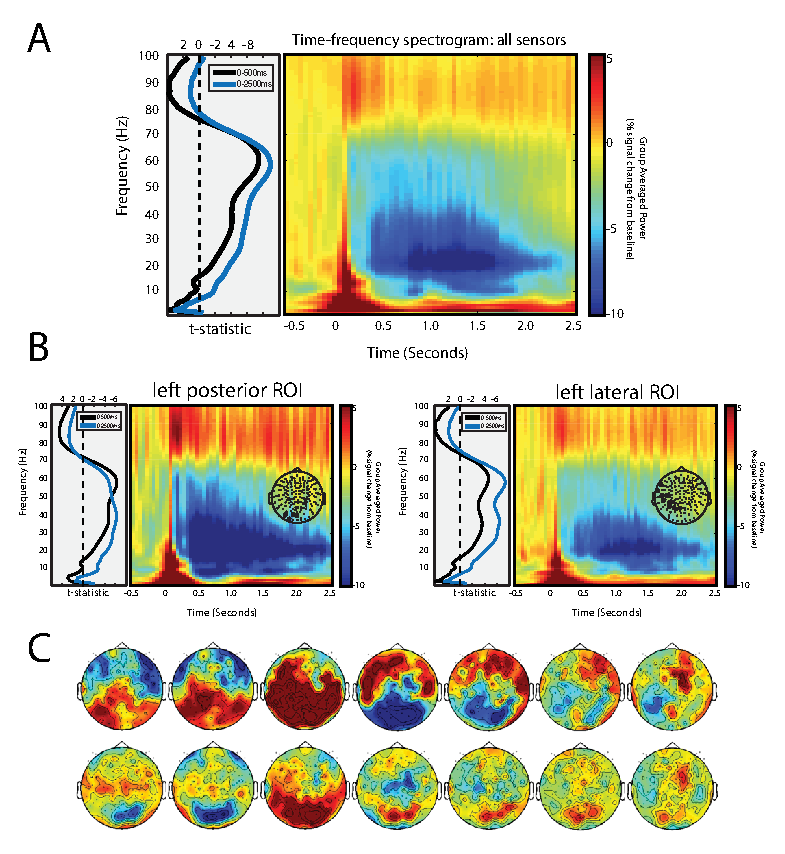
\includegraphics[width=.75\textwidth]{figures/chapter3_suppfigure1.eps}
  \caption[Time-frequency power during stimulus presentation]{\textit{Time-frequency power during stimulus presentation.} (A) Average time-frequency spectrogram is plotted across all sensors and all subjects, where 0 represents stimulus onset.  Power is calculated relative to a pre-stimulus baseline (-1 to -.5).  The line plots on the left side are group-level t-values representing the statistical contrast of the stimulus on period versus the pre-stimulus baseline. The black line represents 0-500ms and the blue line represents 0-2500ms (i.e. the duration of the stimulus on period). (B) Time-frequency power is plotted specifically for the two clusters of sensors that showed the pattern of decreasing theta-gamma coupling by sequence position.  (C) Topographic plots in time bins of 500ms during stimulus presentation.  The top row is theta power and the bottom row is gamma power. }
  \label{chapter3_suppfigure1}
\end{figure}

\begin{figure}
  \centering
  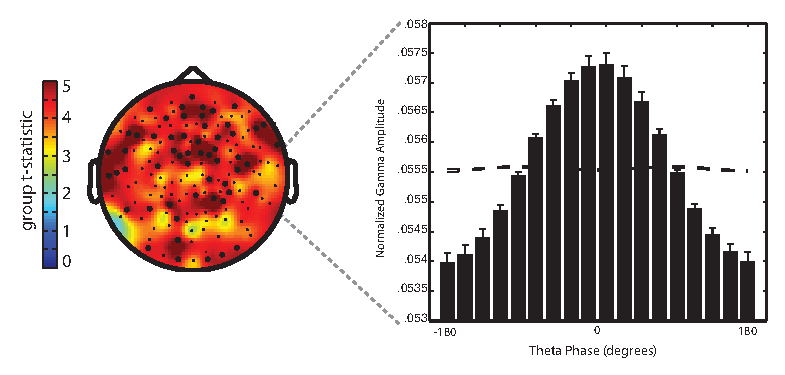
\includegraphics[width=\textwidth]{figures/chapter3_suppfigure2.eps}
  \caption[Theta-gamma coupling across all sensors]{\textit{Theta-gamma coupling across all sensors.} (Left) Topographic plot of group-level t-statistics representing sensors that showed significant theta-gamma coupling during the sequence encoding task (0-2.5 seconds; t(16)>3.96, p<.001).  Filled circles on the topographic plot represent significant sensors. (Right) Gamma power binned by theta phase for sensors that showed significant theta-gamma coupling.  Error bars represent standard error of the group mean.  The dotted lines represent the standard error of the mean of the permuted coupling scores (see Methods for details).}
  \label{chapter3_suppfigure2}
\end{figure}

\begin{figure}
  \centering
  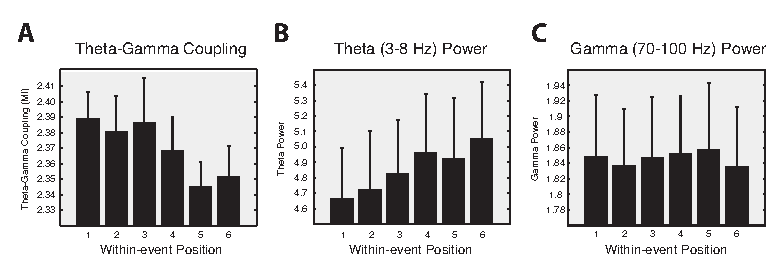
\includegraphics[width=\textwidth]{figures/chapter3_suppfigure3.eps}
  \caption[Power and coupling averaged across significant clusters of sensors]{\textit{Power and coupling averaged across significant clusters of sensors.} (A) Bar graph representing magnitude of theta-gamma coupling (MI or ‘modulation index’) by sequence position averaged across sensors that displayed a significant fit to theta-gamma model.  (B) Theta power by sequence position averaged across sensors displaying significant fit to theta-gamma model. (C) Gamma power by sequence position averaged across sensors displaying significant fit to theta-gamma model.  Error bars represent standard error of the mean.}
  \label{chapter3_suppfigure3}
\end{figure}

\begin{figure}
  \centering
  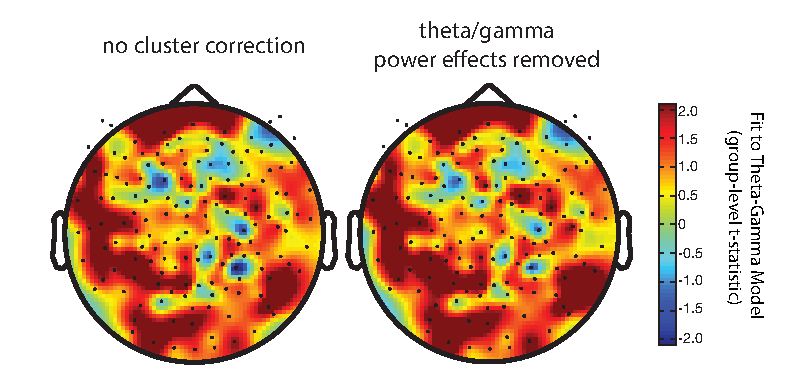
\includegraphics[width=\textwidth]{figures/chapter3_suppfigure4.eps}
  \caption[Decreasing theta-gamma PAC by sequence position model fit data and control analyses]{\textit{Decreasing theta-gamma PAC by sequence position model fit data and control analyses.} The left topographic plot is a statistical plot representing the fit of the theta-gamma model prediction to the theta-gamma coupling data prior to applying the cluster threshold (i.e. Figure 1d before cluster correction, See Methods for details of cluster size permutation procedure).  The right topographic plot represents the result of an analysis where power effects in the theta and gamma band were first regressed out of the theta-gamma coupling data and then the residuals of this analysis were fit to the predicted pattern from the theta-gamma model.}
  \label{chapter3_suppfigure4}
\end{figure}

\begin{figure}
  \centering
  \includegraphics[width=\textwidth]{figures/chapter3_suppfigure5.eps}
  \caption[Source localization analysis with various statistical thresholds]{\textit{Source localization analysis with various statistical thresholds.} The statistical maps represent the group-level fit of the decreasing PAC by sequence position model to the theta-gamma coupling data at various thresholds (p<.001, .01 .1, all uncorrected).  Coronal slices are on the top row, axial slices in the middle row, and sagittal slices are along the bottom row.}
  \label{chapter3_suppfigure5}
\end{figure}

\begin{figure}
  \centering
  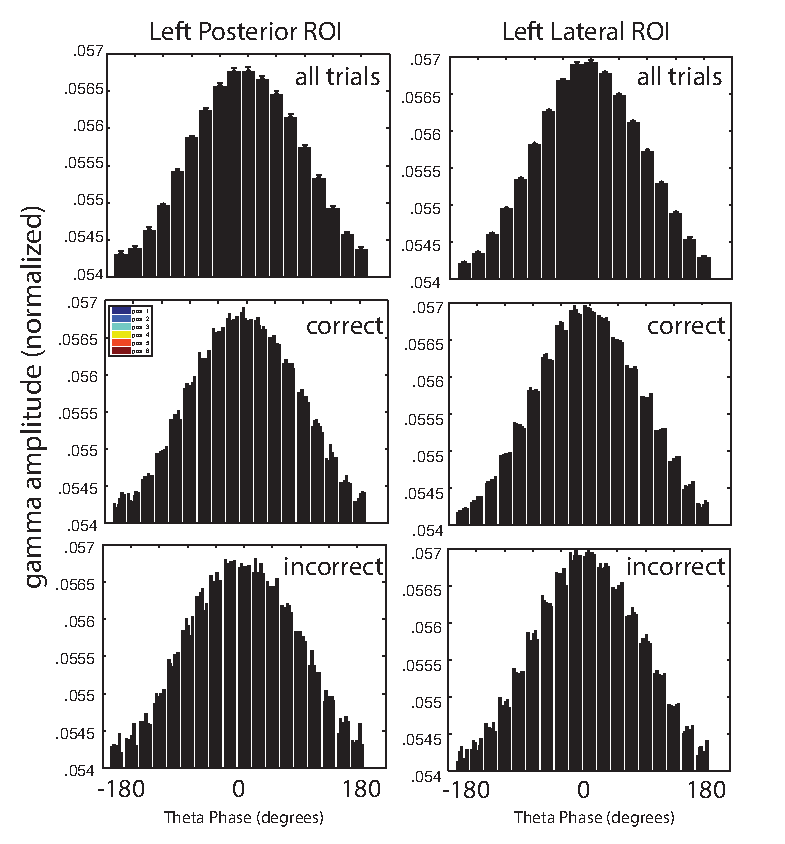
\includegraphics[width=\textwidth]{figures/chapter3_suppfigure6.eps}
  \caption[Group-averaged gamma power binned by theta phase for regions of interest]{\textit{Group-averaged gamma power binned by theta phase for regions of interest.} The two clusters of sensors that showed a significant fit to the decreasing theta-gamma PAC by sequence position model.  On the left, data was extracted from the left posterior cluster of sensors that significantly fit the model of decreasing phase amplitude coupling.  On the top is the group-average across all trials (i.e. irrespective of sequence position).  In the middle, theta-gamma coupling is plotted as a function of sequence position only for trials where the order was later correct and on the bottom, only for trials where the order was later incorrect.  The plots on the right are the same as the left, but for the left lateral cluster of interest.}
  \label{chapter3_suppfigure6}
\end{figure}

\begin{figure}
  \centering
  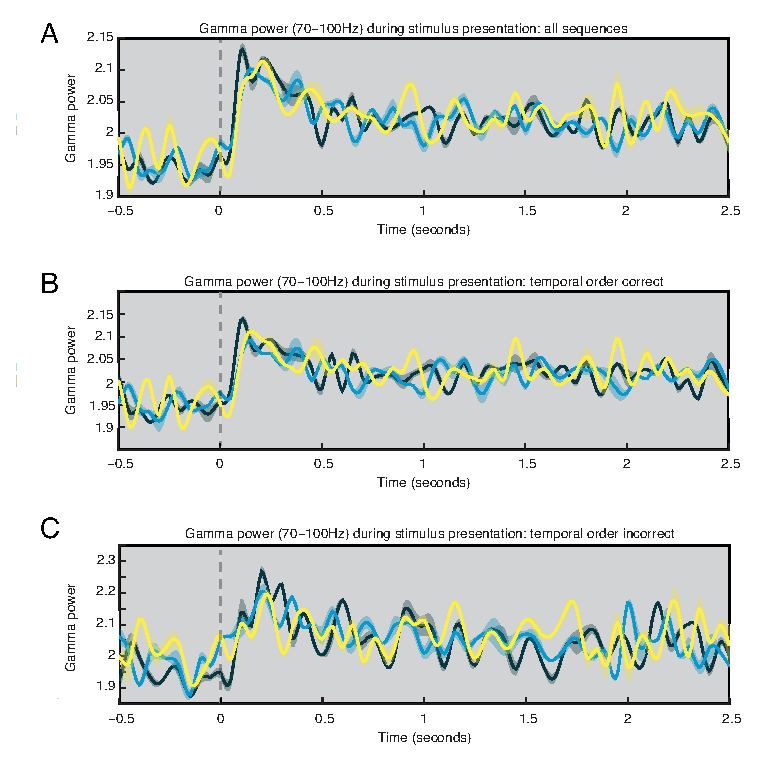
\includegraphics[width=\textwidth]{figures/chapter3_suppfigure7.eps}
  \caption[Gamma power during stimulus presentation]{\textit{Gamma power (70-100 Hz) during stimulus presentation.} (A) Group-averaged time course of gamma power (-.5 to 2.5 seconds) in left posterior cluster of interest for early (dark gray; sequence positions 1 and 2), middle (blue; 3 and 4) and later (yellow; 5 and 6) sequence positions. B) Same as A but for only correctly remembered sequences. (C) Same as A but only for incorrect sequences.  Error bars represent standard error of the mean.}
  \label{chapter3_suppfigure7}
\end{figure}

\begin{figure}
  \centering
  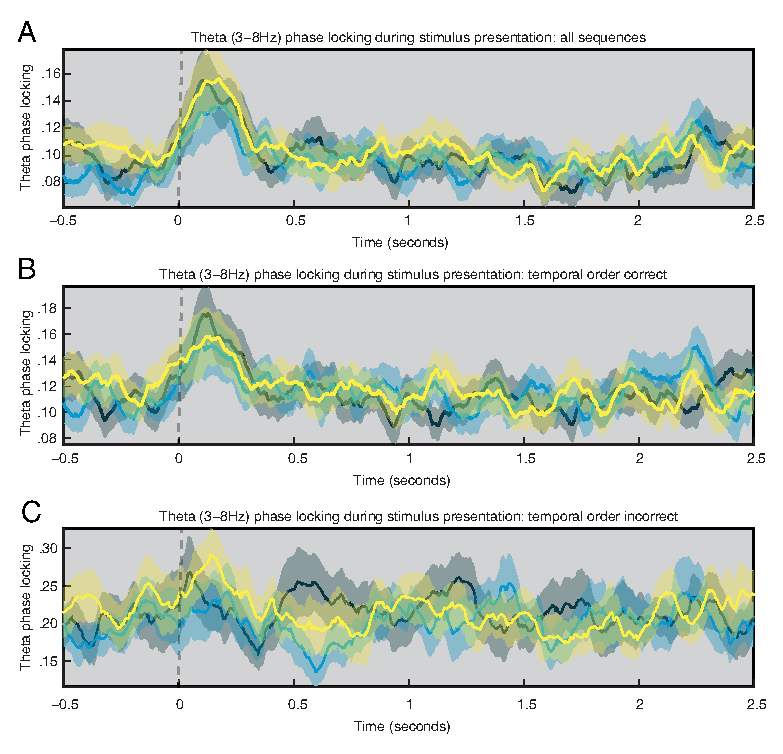
\includegraphics[width=\textwidth]{figures/chapter3_suppfigure8.eps}
  \caption[Theta phase locking during stimulus presentation.]{\textit{Theta phase locking (3-8 Hz) during stimulus presentation.} (A) Group-averaged time course of theta phase locking (-.5 to 2.5 seconds) in left posterior cluster of interest for early (dark gray; sequence positions 1 and 2), middle (blue; 3 and 4) and later (yellow; 5 and 6) sequence positions. (B) Same as A but for only correctly remembered sequences. (C) Same as A but only for incorrect sequences.  Error bars represent standard error of the mean.}
  \label{chapter3_suppfigure8}
\end{figure}

\begin{figure}
  \centering
  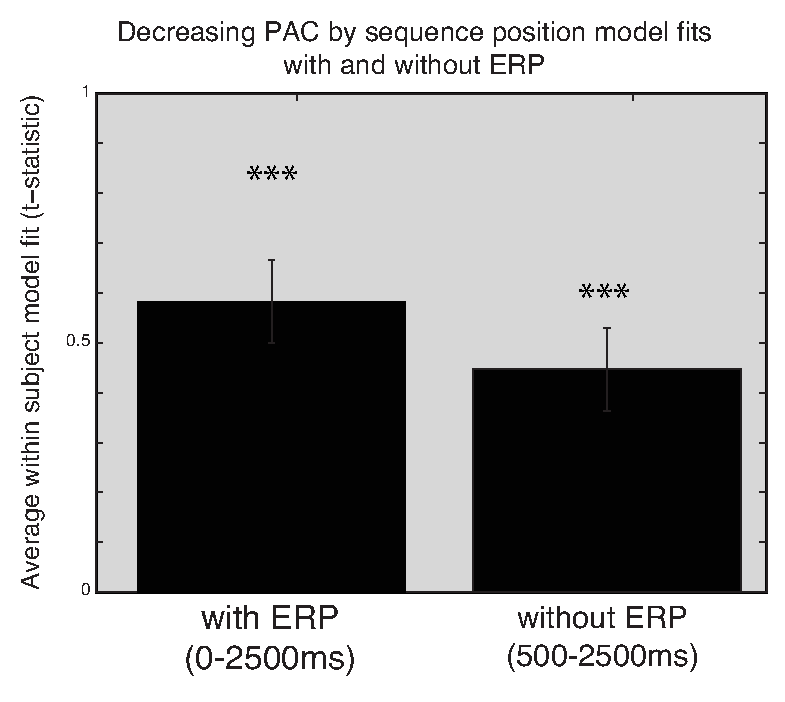
\includegraphics[width=.75\textwidth]{figures/chapter3_suppfigure9.eps}
  \caption[Model fit without ERP]{\textit{Model fit without ERP.} This bar graph depicts the average model fit statistic for a linear decrease in theta-gamma PAC by sequence position, averaging over sensors that showed a significant group-level model fit.  The bar on the left represents the average model fit for the original analysis on the entire stimulus presentation (0-2500ms).  The bar on the right represents the average model fit for the new analysis where we remove the first 500ms (500-2500ms), eliminating the possible contribution of the evoked response.  *** p<.001.}
  \label{chapter3_suppfigure9}
\end{figure}

\begin{figure}
  \centering
  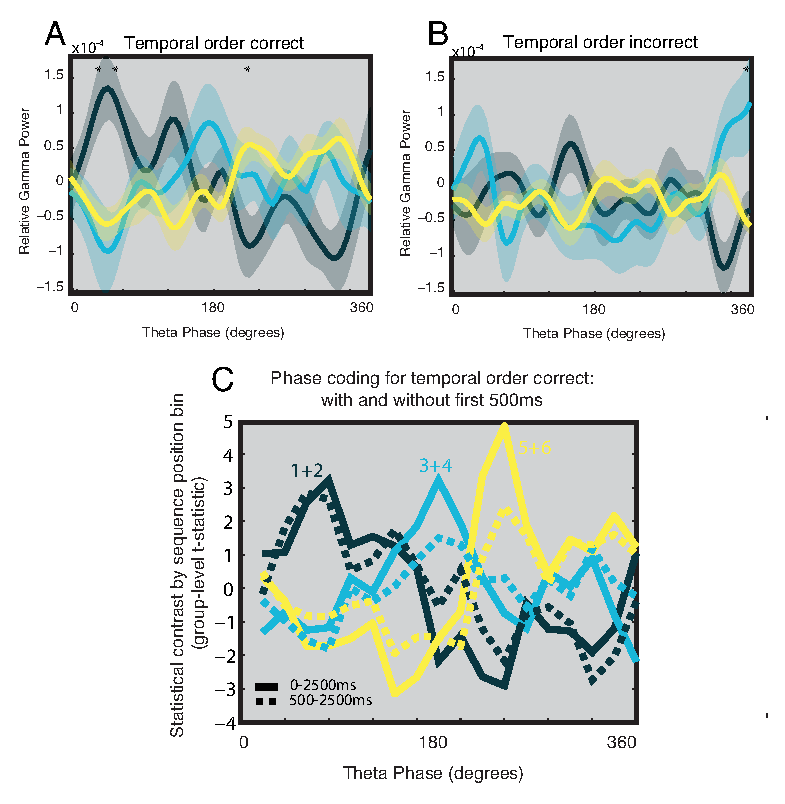
\includegraphics[width=\textwidth]{figures/chapter3_suppfigure10.eps}
  \caption[Phase coding plots without ERP]{\textit{Phase coding plots without ERP.}  Distribution of gamma power over theta phase by sequence position bin for only correctly remembered sequences (Watson William’s Test F(5,96)=9.10, p<.0001). B) Distribution of gamma power over theta phase by sequence position bin for incorrectly remembered sequences (Watson William’s Test F(5,96)=6.42, p<.001). Sequence by position interaction is significant (Harrison-Kanji Test: F(5,196)=11.03, p=.025). C) Group-level statistics for theta phase coding effect with (solid line) and without first 500ms (dashed line). p<.05}
  \label{chapter3_suppfigure10}
\end{figure}

\begin{figure}
  \centering
  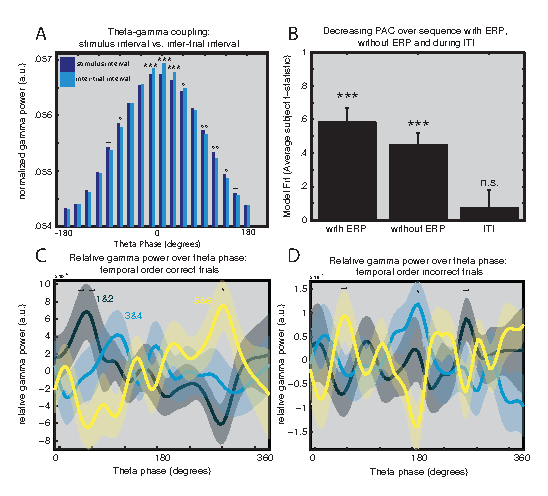
\includegraphics[width=\textwidth]{figures/chapter3_suppfigure11.eps}
  \caption[Theta-gamma coupling during inter-trial interval]{\textit{Theta-gamma coupling during inter-trial interval (ITI; 2500-5000 post stimulus duration).} Histogram of gamma power over theta phase for the stimulus presentation interval (dark blue) and the ITI (light blue). (B) Decreasing PAC by sequence position model fits during the entire stimulus interval, after removing the first 500ms and during the ITI. (C) Distribution of gamma power over theta by sequence position for correct order sequences during the ITI (Watson William’s Test F(5,96)=9.10, p<.0001). (D) Distribution of gamma power over theta by sequence position for incorrect sequences during the ITI (Test F(5,96)=9.09, p<.0001). Sequence by position interaction trending (F(5,196)=8.02, p=.07). ~ p<.1, * p<.05, ** p<.01, *** p<.001.}
  \label{chapter3_suppfigure11}
\end{figure}

\begin{figure}
  \centering
  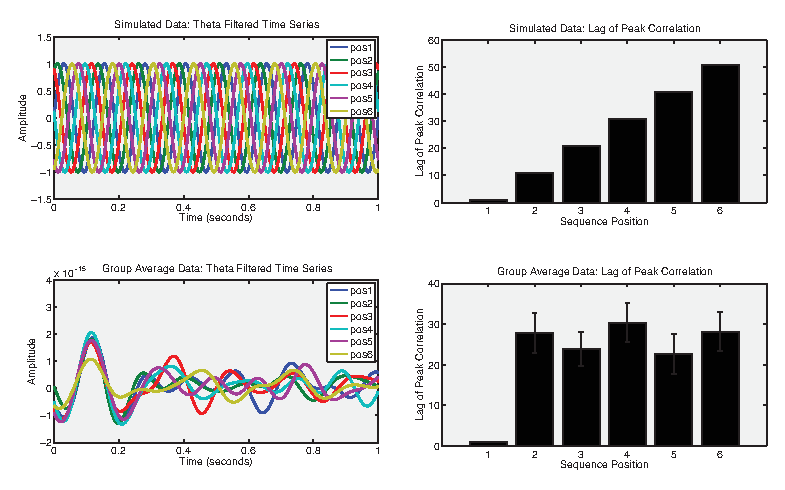
\includegraphics[width=\textwidth]{figures/chapter3_suppfigure12.eps}
  \caption[Testing for systematic theta phase shift by sequence position.]{\textit{Testing for systematic theta phase shift by sequence position.} The top row is simulated data in the theta frequency for each sequence position, where we simulated a systematic linear phase shift over the sequence.  The bottom row is the group-averaged data after computing each of these metrics within-subject.  The left column is the data filtered in the theta band. The right row is the lag of the peak in the pair-wise cross-correlation.  If a systematic phase shift was present in the data, we would expect a monotonically increasing lag as a function of sequence position.}
  \label{chapter3_suppfigure12}
\end{figure}

\begin{figure}
  \centering
  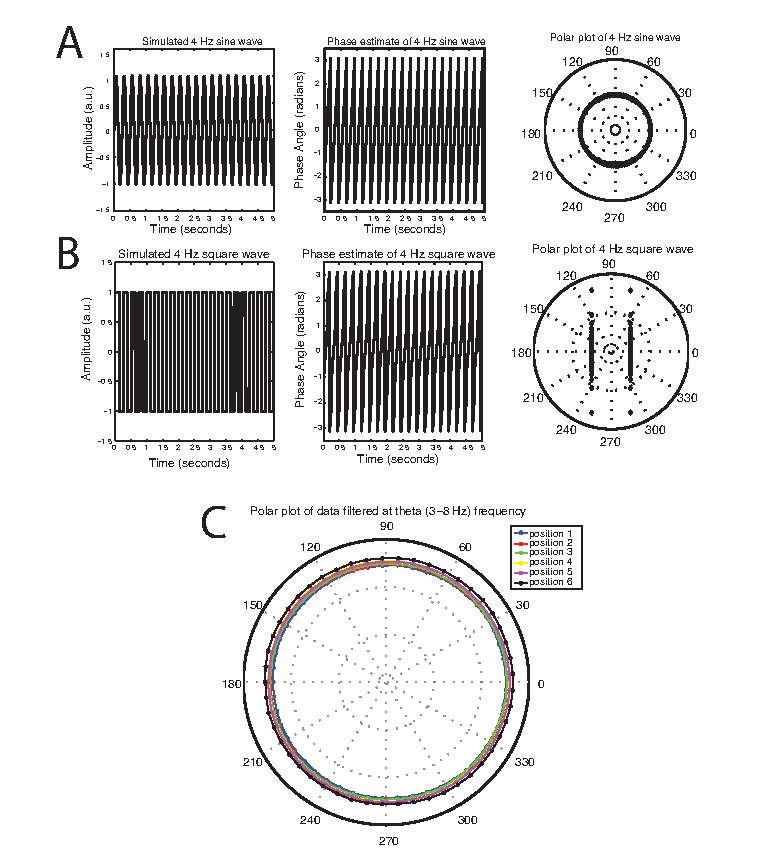
\includegraphics[width=.75\textwidth]{figures/chapter3_suppfigure13.eps}
  \caption[Theta phase symmetry]{\textit{Theta (3-8 Hz) is symmetric and symmetry doesn’t vary by sequence position.} (A) On the left is a simulated 4 Hz sine wave.  Plotted in the middle is the phase time series of the theta wave.  On the right, the waveform is plotted in polar coordinates, where the circular angle represents the phase and the distance from the center represents the power. (B) The same plot as listed above, but for a square wave at 4 Hz. (C) Polar plot representing the grand average of the MEG time series during stimulus presentation (0 to 2.5s) filtered in the theta range (3-8 Hz) and averaged over the left posterior cluster of sensors.  Each color represents a distinct sequence position.}
  \label{chapter3_suppfigure13}
\end{figure}
